\documentclass[12pt,a4paper]{article}

\usepackage{float}
\usepackage{placeins}
\usepackage{amsmath}
\usepackage{color}
\usepackage{amssymb}
\usepackage{mathtools}
\usepackage{subfigure}
\usepackage{multirow}
\usepackage{epsfig}
\usepackage{listings}
\usepackage{enumitem}
\usepackage{graphicx}    
\usepackage{graphics}
\usepackage{epstopdf}
\usepackage{longtable}
\usepackage[pdftex]{hyperref}
\usepackage{breakurl}
\usepackage{epigraph}
\usepackage{xspace}
\usepackage{amsfonts}
\usepackage{eurosym}
\usepackage{ulem}
\usepackage{footmisc}
\usepackage{comment}
\usepackage{sectsty}
\usepackage{setspace}
\usepackage{geometry}
\usepackage{caption}
\usepackage{pdflscape}
\usepackage{array}
\usepackage[round]{natbib}
\usepackage{booktabs}
\usepackage{dcolumn}
%\usepackage[justification=centering]{caption}
%\captionsetup[table]{format=plain,labelformat=simple,labelsep=period,singlelinecheck=true}%

%\bibliographystyle{unsrtnat}
\bibliographystyle{aea}
\usepackage{enumitem}
%\usepackage{tikz}
%\usetikzlibrary{snakes}
%\usetikzlibrary{patterns}

\normalem

\doublespacing
\newtheorem{theorem}{Theorem}
\newtheorem{corollary}[theorem]{Corollary}
\newtheorem{proposition}{Proposition}
\newenvironment{proof}[1][Proof]{\noindent\textbf{#1.} }{\ \rule{0.5em}{0.5em}}
\newcommand{\ra}[1]{\renewcommand{\arraystretch}{#1}}

\newcolumntype{d}[1]{D{.}{.}{#1}} % "decimal" column type
\renewcommand{\ast}{{}^{\textstyle *}} % for raised "asterisks"

\newtheorem{hyp}{Hypothesis}
\newtheorem{subhyp}{Hypothesis}[hyp]
\renewcommand{\thesubhyp}{\thehyp\alph{subhyp}}

\newcommand{\red}[1]{{\color{red} #1}}
\newcommand{\blue}[1]{{\color{blue} #1}}

\newcommand*{\qed}{\hfill\ensuremath{\blacksquare}}%

\newcolumntype{L}[1]{>{\raggedright\let\newline\\arraybackslash\hspace{0pt}}m{#1}}
\newcolumntype{C}[1]{>{\centering\let\newline\\arraybackslash\hspace{0pt}}m{#1}}
\newcolumntype{R}[1]{>{\raggedleft\let\newline\\arraybackslash\hspace{0pt}}m{#1}}

\geometry{left=1.0in,right=1.0in,top=1.0in,bottom=1.0in}

\epstopdfsetup{outdir=./}

\newcommand{\elabel}[1]{\label{eq:#1}}
\newcommand{\eref}[1]{Eq.~(\ref{eq:#1})}
\newcommand{\ceref}[2]{(\ref{eq:#1}#2)}
\newcommand{\Eref}[1]{Equation~(\ref{eq:#1})}
\newcommand{\erefs}[2]{Eqs.~(\ref{eq:#1}--\ref{eq:#2})}

\newcommand{\Sref}[1]{Section~\ref{sec:#1}}
\newcommand{\sref}[1]{Sec.~\ref{sec:#1}}

\newcommand{\Pref}[1]{Proposition~\ref{prop:#1}}
\newcommand{\pref}[1]{Prop.~\ref{prop:#1}}
\newcommand{\preflong}[1]{proposition~\ref{prop:#1}}

\newcommand{\clabel}[1]{\label{coro:#1}}
\newcommand{\Cref}[1]{Corollary~\ref{coro:#1}}
\newcommand{\cref}[1]{Cor.~\ref{coro:#1}}
\newcommand{\creflong}[1]{corollary~\ref{coro:#1}}

\newcommand{\etal}{{\it et~al.}\xspace}
\newcommand{\ie}{{\it i.e.}\ }
\newcommand{\eg}{{\it e.g.}\ }
\newcommand{\etc}{{\it etc.}\ }
\newcommand{\cf}{{\it c.f.}\ }
\newcommand{\ave}[1]{\left\langle#1 \right\rangle}
\newcommand{\person}[1]{{\it \sc #1}}

\newcommand{\AAA}[1]{\red{{\it AA: #1 AA}}}
\newcommand{\YB}[1]{{\it YB: #1 YB}}

\newcommand{\flabel}[1]{\label{fig:#1}}
\newcommand{\fref}[1]{Fig.~\ref{fig:#1}}
\newcommand{\Fref}[1]{Figure~\ref{fig:#1}}

\newcommand{\tlabel}[1]{\label{tab:#1}}
\newcommand{\tref}[1]{Tab.~\ref{tab:#1}}
\newcommand{\Tref}[1]{Table~\ref{tab:#1}}

\newcommand{\be}{\begin{equation}}
\newcommand{\ee}{\end{equation}}
\newcommand{\bea}{\begin{eqnarray*}}
\newcommand{\eea}{\end{eqnarray*}}

\newcommand{\bi}{\begin{itemize}}
\newcommand{\ei}{\end{itemize}}

\newcommand{\Dt}{\Delta t}
\newcommand{\etau}{\tau^\text{eqm}}
\newcommand{\wtau}{\widetilde{\tau}}
\newcommand{\xN}{\ave{x}_N}
\newcommand{\Sdata}{S^{\text{data}}}
\newcommand{\Smodel}{S^{\text{model}}}

\numberwithin{equation}{section}
\DeclareMathOperator\erf{erf}
%\let\endtitlepage\relax
\begin{document}

\onehalfspacing

\begin{titlepage}
\title{The relationship between relative and absolute mobility -- theory and empirics}
\author{Yonatan Berman\footnote{Paris School of Economics, Paris, France, yonatan.berman@psemail.eu}\, and Alexander Adamou\footnote{London Mathematical Laboratory, London, UK, a.adamou@lml.org.uk} \thanks{We wish to thank Tslil Aloni, Mikkel H\o st Gandil, Ole Peters, Yoash Shapira and Alex Teytelboym for fruitful discussions and for their feedback on the manuscript.}}
\date{Original version: June 20, 2017\,\,\,\,\,\,\,\,\,\,\,\,\,\,\,\,\,\,\,\,\,\,\,\,Last updated: \today}
%\date{Last updated: \today}
\maketitle
\begin{abstract}
\noindent~\citet{chetty2014land} proposed a new measure of absolute intergenerational income mobility: the fraction of children with greater real-terms income than their parents.~\citet{chetty2017fading} studied this empirically using United States income data. They found that this measure of absolute income mobility has decreased over the last four decades. %while traditional measures of relative income mobility have remained largely stable.
They explained this as a consequence of unequal income growth. Here we establish an analytical relationship between their absolute mobility measure and traditional measures of relative mobility. % in a model in which parent and child log-incomes follow a bivariate normal distribution.
We find that the absolute mobility measure is, ceteris paribus, inversely related to traditional relative mobility measures. Additionally, our model suggests mechanisms by which changes in the marginal distributions of parent and child incomes influence absolute mobility. Our findings also offer a way to estimate absolute intergenerational mobility based on existing data on relative intergenerational mobility and on income distributions without the need for high-quality panel data sets unavailable in many countries.
%Our results are generalisable to other joint distributions of parent and child income.
\\
\\
\noindent\textbf{Keywords:} Mobility, inequality, bivariate income distributions, copula modeling
\\
\noindent\textbf{JEL Codes:} E0, H0, J0, R0\\

\bigskip
\end{abstract}
\setcounter{page}{0}
\thispagestyle{empty}
%\nopagebreak
\end{titlepage}
\pagebreak \newpage
%\nopagebreak

\doublespacing

\section{Introduction} \label{sec:introduction}

The ``growing public perception that intergenerational income mobility [\ldots] is declining in the United States''~\citep[p.~141]{chetty2014united} has led scholars to seek quantifiable measures of it. Typically such measures are divided into two classes: relative and absolute. Relative measures gauge children's propensity to occupy a different position in the income distribution than their parents. Absolute measures gauge their propensity to have higher incomes than their parents in real terms. A hypothetical economy in which all children have exactly twice the real incomes of their parents would exhibit minimal relative mobility and maximal absolute mobility. 

Different mobility measures ``capture different normative concepts''~\citep[p.~1560]{chetty2014land} and, therefore, may create different and possibly contradictory pictures of ostensibly the same phenomenon. At worst, this misleads the unaware. At best, it complicates analysis. The root of the problem is that ``attaching a precise normative significance to `income mobility' is difficult because of the multidimensionality of this concept''~\citep[p.~588]{fields1999measurement}. In other words, mobility is not simply defined.

While relative intergenerational income mobility has been studied for decades~\citep{becker1979equilibrium,borjas1992ethnic,piketty2000theories,mazumder2005fortunate,aaronson2008intergenerational,lee2009trends,hauser2010intergenerational,corak2013income,chetty2014united,berman2016understanding}, investigations of absolute intergenerational income mobility remain ``scarce, mainly because of the lack of large, high-quality panel data sets linking children to their parents''~\citep[p.~398]{chetty2017fading}. \citet[p.~1563]{chetty2014land} introduced a new measure of absolute mobility: the fraction of children with higher inflation-adjusted incomes than their parents at the same age, which we denote by $A$. \citet{chetty2017fading} considered historical trends in $A$ in the United States, finding that it has fallen from around 90\% for children born in 1940 to 50\% for children born in the 1980s (see \fref{trend}). These findings are consistent with the study by \citet{isaacs2007economic}.
%Based on the~\citet{PSID2017},~\citet{isaacs2007economic} found that ``$67\%$ percent of Americans had higher levels of family incomes than their own parents'' (for children born during the 1950s and 1960s), agreeing with the values reported by~\citet{chetty2017fading}.

\begin{figure}[!htb]
\centering
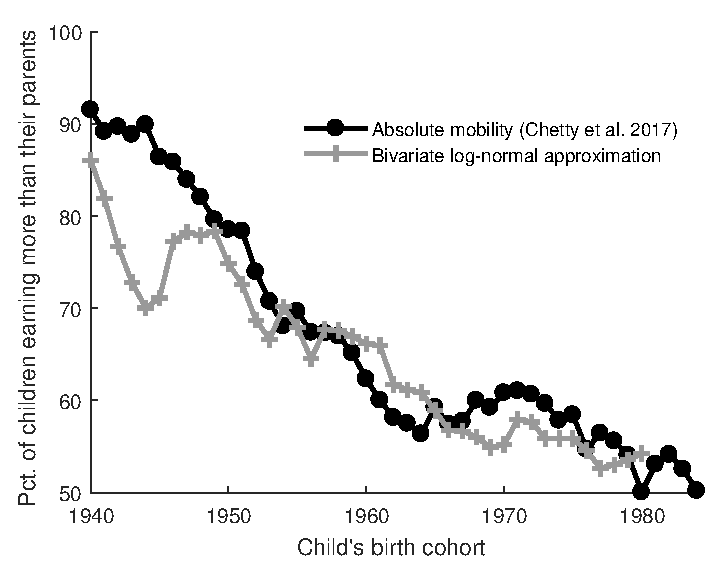
\includegraphics[width=1.0\textwidth] {./figs/trend2.eps}
\caption{A comparison between the measured (black) and approximated absolute mobility (gray). A bivariate normal distribution reproduces the historical trend of the rate of absolute mobility (the calculations are based on the pre-tax national income per adult and pre-tax income distribution reported in~\citet{WID2017} assuming fixed correlation of $\rho=0.313$). The correlation coefficient between the measured and approximated time series was $0.91$. \AAA{The zooming on the vertical axis magnifies the 1940s discrepancy. Also, why does the grey line stop before the black line?} 
}
\flabel{trend}
\end{figure}

The canonical measure of relative intergenerational mobility is the elasticity of the logarithm of child income with respect to the logarithm of parent income.\footnote{Dimensional analysis requires that physically meaningful quantities have dimension functions which are power-law monomials~\citep{barenblatt2003}. Therefore, while an income measured in dollars per year is physically meaningful, its logarithm is not. Strictly speaking, we are using ``log-income'' here as a shorthand for the logarithm of the dimensionless ratio of observed income to a base unit of income of \$1 per year.} This is known as the intergenerational earnings elasticity (IGE)~\citep{mulligan1997parental,lee2009trends,chetty2014land} and we denote it by $\beta$. IGE is a measure of immobility rather than of mobility: the larger it is, the stronger the relationship between parent and child incomes. Therefore, $R_1 \equiv 1-\beta$ is used as a measure of relative mobility. Unlike absolute mobility, most empirical studies of IGE and other relative mobility measures in the United States show them holding stable over recent decades~\citep{lee2009trends,hauser2010intergenerational,chetty2014land,chetty2014united}. 

Another common measure of relative mobility is the rank-rank slope (RRS), defined as the slope of the straight line found by ``regressing the child's rank on his parents' rank'' in their marginal income distributions~\citep[p.~1561]{chetty2014land}. We denote it by $\rho_S$. \AAA{Maybe change this, e.g. to $\gamma$, to avoid confusion with correlation coefficients?} As a rank-based measure, RRS depends only on the copula of the joint income distribution of parents and children, whereas IGE depends additionally on the standard deviation of the log-incomes. \citet[p.~1561]{chetty2014land} argued that rank-rank slopes ``prove to be much more robust across specifications and are thus more suitable for comparisons across areas from a statistical perspective''. Similarly to IGE, the RRS is also a measure of immobility, and we use $R_2 \equiv 1-\rho_S$ as the corresponding measure of relative mobility.

Co-observations of declining absolute mobility and stable relative mobility require careful interpretation. \citet{chetty2017fading} explain them as a consequence of unequally distributed income growth. When growth is positive for high earners and stagnant for the rest, aggregate income growth contributes little to absolute mobility. This narrative is consistent with their data but, as we show here, it may not describe the only mechanism at work.

We present a theoretical study of the absolute mobility measure $A$, with particular focus on the relationship between $A$ and the two measures of relative mobility, $R_1$ and $R_2$. We find, in a simple and plausible model of the joint log-income distribution, that absolute mobility is inversely related to both relative mobility measures. The finding proves robust over different copula families and marginal distributions.

Although \citet[p.~1574]{chetty2014land} argued that ``the income distribution is not well approximated by a bivariate log-normal distribution'', we find that the decline in absolute mobility in the United States is. No other choice of copula and marginal distribution resulted in a better description of this trend.

Using the bivariate normal model, it is possible to obtain closed-form expressions for the dependencies of $A$ on $R_1$ and on $R_2$. This helps elucidate possible mechanisms by which changes in the marginal distributions of parent and child incomes influence absolute mobility, whose discussion has been hitherto limited.

Our contribution is threefold. Firstly, we offer the first theoretical study of the relationship between the canonical measures of intergenerational income mobility. We suggest that their co-movement should not, in general, be expected.

Secondly, we show empirically that a simple model of a bivariate log-normal income distribution can describe adequately the long run dynamics of absolute mobility. This unlocks powerful theoretical and empirical techniques. In particular, the log-normal distribution is that of random multiplicative growth, which suggests connections to generative models of income and wealth whose use is often prohibited by assumptions of ergodicity~\citep{adamou2016,berman2016far}.

Thirdly, we find that data on marginal income distributions and relative intergenerational mobility, which are widely available, can be used to estimate absolute intergenerational mobility without the need for the additional high-quality panel data sets, which are usually required and which remain unavailable for most countries.

\section{Model}

Our starting point is a population of $N$ parent-child pairs. We denote by $Y_p^i$ and $Y_c^i$ the respective \AAA{inflation-adjusted?} incomes of the parent and the child (at the same age) in family $i=1\dots N$. We assume the incomes are all positive and define the log-incomes $X_p^i=\log Y_p^i$ and $X_c^i=\log Y_c^i$.

The intergenerational earnings elasticity is defined as the slope ($\beta$) of the linear regression
\be
X_c = \alpha + \beta X_p + \epsilon\,,
\ee
where $\alpha$ is the regression intercept and $\epsilon$ is the error term. We define $R_1\equiv 1- \beta$ as the corresponding measure of intergenerational mobility.

The rank-rank slope
%(sometimes called the rank-rank correlation or Spearman's $\rho$) is defined as the correlation coefficient 
is defined as the slope of the linear regression of the child percentile ranks on the parent percentile ranks in their respective marginal income distributions. We denote it by $\rho_S$ and define $R_2\equiv 1- \rho_S$ as the corresponding measure of intergenerational mobility.

The rate of absolute mobility, $A$, introduced in~\citep[p.~1563]{chetty2014land} is the fraction of children earning more than their parents in real terms, equal to the probability $P\left(X_c-X_p > 0\right)$.

One hypothetical sample of the joint parents and children log-income distribution is presented in~\fref{lines}.~\fref{lines} also depicts how $A$ and $\beta$ are defined -- the blue line is $y=x$, hence the rate of absolute mobility is defined as the fraction of parent-child pairs which are above it. The red line is the linear regression $y=\alpha +\beta x$, for which $\beta$ is the IGE.

\begin{figure}[!htb]
\centering
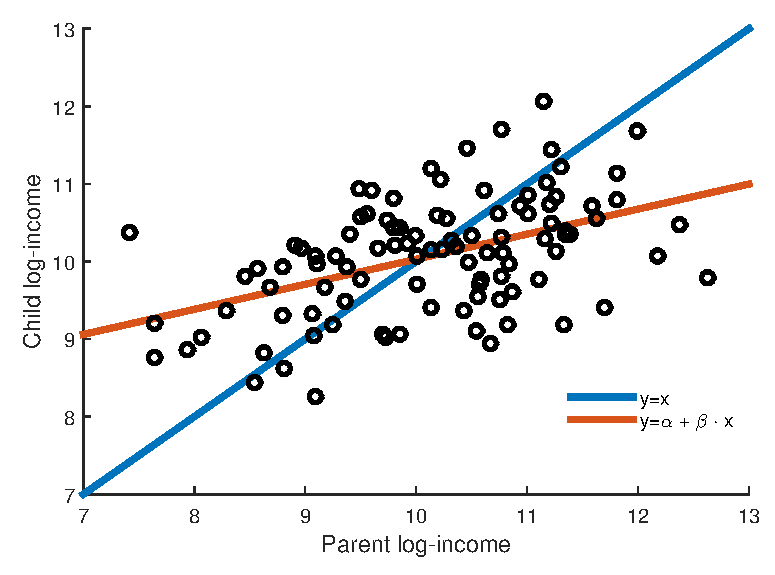
\includegraphics[width=1.0\textwidth]{./figs/bivariate_lines3.eps}
\caption{An illustration of the absolute and relative mobility measures. The black circles are a randomly chosen sample of 100 parent-child log-income pairs, assuming a bivariate normal distribution. The parameters used were $\mu_p=10.1$, $\sigma_p=0.78$ (for the parents marginal distribution) and $\mu_c=10.25$, $\sigma_c=1.15$ (for the children marginal distribution) with correlation of $\rho=0.6$. The resulting $\alpha$ and $\beta$ were $1.8$ and $0.84$, respectively.}
\flabel{lines}
\end{figure}

The log-normal distribution is a good approximation of empirical income distributions~\citep{pinkovskiy2009parametric} and has a mechanistic basis as the long-run attractor distribution for quantities undergoing random multiplicative growth~\cite{aitchison1957,adamou2016}. Thus, a simple and plausible model for the joint distribution of parent and child log-incomes is the bivariate normal distribution. In this model, the marginal income distributions of both parents and children are log-normal and the correlation between their log-incomes is defined by a single parameter $\rho$. The marginal log-income distributions of the parents and the children follow $\mathcal{N}\left(\mu_p,\sigma_p^2\right)$ and $\mathcal{N}\left(\mu_c,\sigma_c^2\right)$, respectively. Hence the joint distribution is fully characterized by 5 parameters: $\mu_p$, $\sigma_p$, $\mu_c$, $\sigma_c$ and $\rho$.

The choice of model may affect the analysis of the absolute and relative mobility measures. Other possible models for the joint income distribution of parents and children can include marginal distributions which are not log-normal, such as beta and gamma distributions, as well as other types of copula. In the bivariate log-normal model the copula is Gaussian, while other types found useful for various empirical applications~\citep{trivedi2007copula}, such as the Clayton, the Gumbel and the Plackett copula families~\citep{bonhomme2009assessing}, may prove to be a better description of the relationship between the marginal income distributions. In their study of intergenerational mobility in France,~\citet{bonhomme2009assessing} argue that the Gaussian copula ``tends to underestimate the dependence in the middle of the distribution, that is, the probabilities of remaining in the second, third, and fourth quintiles'' and show that the empirical copula is best estimated by the Plackett copula. In Appendix~\ref{app:appB} we show that the bivariate log-normal model with Gaussian copula reproduces the measured historical trend of absolute mobility in the United States at least as well as the other models tested. \AAA{I feel this paragraph would be better placed in an appendix. Primarily these are fitting exercises to demonstrate the adequacy of our chosen model. The lognormal distribution has a dynamical basis (as we now point out in the text) whereas these other distributions do not.}

\section{Results}
\label{sec:results}

We first address the properties of the bivariate log-normal approximation. We derive closed-form expressions for the measures of mobility -- $A$, $R_1$, and $R_2$ -- in terms of the model distribution parameters.

\begin{proposition}
\label{prop:prop1}

For a bivariate normal distribution with parameters $\mu_p$, $\sigma_p$ (for the parents marginal distribution) and $\mu_c$, $\sigma_c$ (for the children marginal distribution) assuming correlation $\rho$, the relative mobility $R_1$ is

\be
R_1 = 1-\frac{\sigma_c}{\sigma_p}\rho \,.
\elabel{beta_rho}
\ee
\end{proposition}

Following \pref{prop1} it is also possible to derive the rate of absolute mobility as a function of the distribution parameters and the IGE:

\begin{proposition}
\label{prop:prop2}

For a bivariate normal distribution with parameters $\mu_p$, $\sigma_p$ (for the parents marginal distribution), $\mu_c$, $\sigma_c$ (for the children marginal distribution) and correlation $\rho$, the rate of absolute mobility is

\be
A = \Phi\left(\frac{\mu_c - \mu_p}{\sqrt{\sigma_p^2\left(2R_1-1\right) + \sigma_c^2}}\right) \,,
\elabel{abs2}
\ee
where $\Phi$ is the cumulative distribution function of the standard normal distribution.
\end{proposition}
\AAA{I changed $\beta$ to $R_1$ here, since the next proposition is expressed in terms of $R_2$ and not $\rho_S$. Does this change have implications elsewhere?}

\Eref{abs2} enables the calculation of $A$ assuming the knowledge of the marginal income distributions and $R_1$ (or $\beta$). It is therefore also possible to calculate $A$ in terms of $R_2$. \AAA{This needs more explanation. Aren't we just inserting the result from \citep{trivedi2007copula} here? Either way, let's explain in simple terms what we're doing.}

\begin{corollary}
\clabel{coro1}

Under~\pref{prop2} notations, the rate of absolute mobility $A$ is

\be
A = \Phi\left(\frac{\mu_c - \mu_p}{\sqrt{\sigma_p^2\left(1 - \frac{4\sigma_c}{\sigma_p}\sin{\left(\frac{\pi\left(1-R_2\right)}{6}\right)}\right) + \sigma_c^2}}\right) \,.
\elabel{abs3}
\ee
where $\Phi$ is the cumulative distribution function of the standard normal distribution.
\end{corollary}

Our next step is to test whether the bivariate log-normal model for the joint income distribution is empirically sound. For that purpose we compare the model prediction for the historical rate of absolute mobility in the United States with the historical rate reported by~\citet{chetty2017fading}.

We use data for the pre-tax national income per adult in the United States and the top $10\%$ income share data~\citep{WID2017} to obtain $\mu_p$, $\sigma_p$, $\mu_c$ and $\sigma_c$ every year. These parameters can be obtained directly as follows. The Lorenz curve of the log-normal distribution, $\log{\mathcal{N}}\left(\mu,\sigma^2\right)$, is~~\citep{cowell2011measuring}
\be
s(z) = \Phi\left(\Phi^{-1}\left(z\right)-\sigma\right),
\ee
where $s$ is the fraction of the total income earned by the bottom fraction $z$ of the population. The top $10\%$ income share data are time series of $1-s(0.9)$ so, rearranging, we can estimate the corresponding time series of $\sigma$ values as
\be
\sigma = \Phi^{-1}\left(0.9\right) - \Phi^{-1}\left(1-s(0.9)\right)\,.
\ee
If we denote the per-capita pre-tax income as $m$, it follows from the properties of the log-normal distribution that the parameter $\mu$ is
\be
\mu = \log{\left(m\right)} - \frac{\sigma^2}{2}\,.
\ee
\AAA{I tried to clarify this paragraph, as I found it too concise to follow easily. It never hurts to spell out manipulations like these. Feel free to edit, as I still think it can be made clearer.}

Using Eqs.~(\ref{eq:beta_rho}--\ref{eq:abs3}) in order to calculate the historical value of $A$ also requires knowing the correlation $\rho$.~\citet{chetty2014united} report a consistent RRS of $0.3$, which corresponds to a fixed value of $\rho=2\sin{\left(0.05\pi\right)}\approx0.313$ (see the proof of~\creflong{coro1} or~\citet{trivedi2007copula} for the relationship between $\rho$ and the RRS).

The gray curve in~\fref{trend} shows that the model reproduces faithfully the evolution of absolute mobility reported by~\citet{chetty2017fading}, despite its comparative methodological na\"{i}vety. The correlation coefficient between the measured and approximated time series was $0.91$. The model only fails in reproducing the reported absolute mobility for the 1940s birth cohorts. A possible explanation is that for these cohorts the value of $\rho$, and hence the IGE and the RRS values, were substantially different from the reported RRS of $0.3$, since this estimation was based only on the $1971$--$1986$ birth cohorts~\citep{chetty2014united}. However, this cannot be the only explanation, since the quoted absolute mobility values are also based on a time-constant RRS~\citep{chetty2017fading}.

In Appendix~\ref{app:appB} we show that our results are robust under different choices of copula and when the gamma distribution approximation for the marginal income distributions is used instead of the log-normal approximation. The choice of copula is of no importance to the values of the absolute mobility. In addition, the log-normal approximation for the marginal distributions provides consistently better results than the gamma distribution approximation. \AAA{I'm a little confused here. As far as I'm aware, the results in \fref{trend} show only the results using the relationship between $A$ and $\beta$. Is that right? If so, then we haven't actually used the copula at all. The copula is needed in our setup only to estimate the RRS, which we've spoken about a lot but done nothing with. Or have we used the copula to estimate the correlation $\rho$? My worry is that this paragraph seems out-of-place if we haven't done much with the copula, but I'm probably missing something here. Please enlighten me!}

\subsection{Absolute mobility and median incomes}

\citet{chetty2017fading} also find that the share of children earning more than the median parent declined from 92\% in the 1940 birth cohort to 45\% in the 1984 cohort~\citep{katz2017documenting}. This alternative measure of absolute mobility moves almost identically to $A$ across cohorts in the United States~\citep{katz2017documenting}. Defining the share of children earning more than the median parent as $\tilde{A}$, it simply follows in the bivariate log-normal model that $\tilde{A}$ is defined as

\be
\tilde{A} \equiv \Phi\left(\frac{\mu_c-\mu_p}{\sigma_c} \right)\,,
\elabel{tildeA}
\ee
where $\Phi$ is the cumulative distribution function of the standard normal distribution.

Using $\tilde{A}$ has obvious advantages over $A$. In particular, they can be ``directly computed from standard public-use cross-sectional household survey data and do not require data that longitudinally link children to parents''~\citep[p.~382]{katz2017documenting}. However, $\tilde{A}$ would be close to $A$ only if the IGE is close to $0.5$:

\begin{proposition}
\label{prop:prop3}

For a bivariate normal distribution with parameters $\mu_p$, $\sigma_p$ (for the parents marginal distribution), $\mu_c$, $\sigma_c$ (for the children marginal distribution) and assuming IGE of $\beta$, then

\be
A=\tilde{A} \iff \beta=\frac{1}{2}\,.
\ee
\end{proposition}

It is therefore no surprise that for the United States $A$ and $\tilde{A}$ are relatively similar --~\citet{aaronson2008intergenerational} estimate the IGE for the $1950$--$1970$ birth cohorts at $0.46$--$0.58$. In countries such as Denmark or Finland, in which the IGE is substantially lower than $0.5$~\citep{corak2013income}, using $\tilde{A}$ neglects the part high relative mobility plays in determining $A$. This will lead to significant overestimation of absolute intergenerational mobility. For example, in Denmark, the average estimated $A$ for $1950$--$1980$ birth cohorts is $78.7\%$ (see~\sref{global}). If $\tilde{A}$ is considered, the average value is $87\%$. For the United States this difference would be considerably smaller: $70.7\%$ and $72.8\%$, respectively. Setting aside the normative question of which measure of absolute intergenerational mobility is of most interest, we emphasize that $\tilde{A}$ cannot be used as a proxy for $A$, unless the IGE is close to $0.5$. \AAA{I wonder whether the claim of the final sentence, which seems relatively minor to me, warrants an entire section of our paper. It feels more like an appendix item or even a footnote. Having it as a section blocks the flow of our arguments. What do you think?}

\subsection{Estimating absolute mobility globally}
\label{sec:global}

Without directly estimating absolute mobility the way done by~\citet{chetty2017fading}, it is possible to use the bivariate log-normal model for describing the dynamics of absolute mobility in many countries under the assumption that their RRS is fixed and is known. Although this seems as a very limiting assumption, in practice, in most cases, the effect of the RRS value on the estimated absolute mobility is relatively mild. A $10\%$ error in the estimation of the RRS yields an error of about $1\%$ in the average estimated absolute mobility for the United States. \AAA{This needs some explanation.} We note, however, that for specific birth cohorts the effect of changing the RRS on the absolute mobility may be dramatic, as described below and illustrated in~\fref{relat}.

Using available data on the marginal income distributions and on relative intergenerational mobility, we demonstrate how one can produce estimates of absolute intergenerational mobility without the need for high-quality panel data sets. Such data sets remain unavailable in most countries. This is depicted in~\fref{countries} for France, Sweden, Denmark and China, in addition to the reproduced absolute mobility in the United States presented above. The calculations are based on the pre-tax national income per adult and the income share data as reported in~\citet{WID2017} and on relative mobility measurements as reported by~\citet{lefranc2005intergenerational} for France, by~\citet{bjorklund1997intergenerational} for Sweden, by~\citet{landerso2016scandinavian} for Denmark and by~\citet{fan2015great} for China.

\begin{figure}[!htb]
\centering
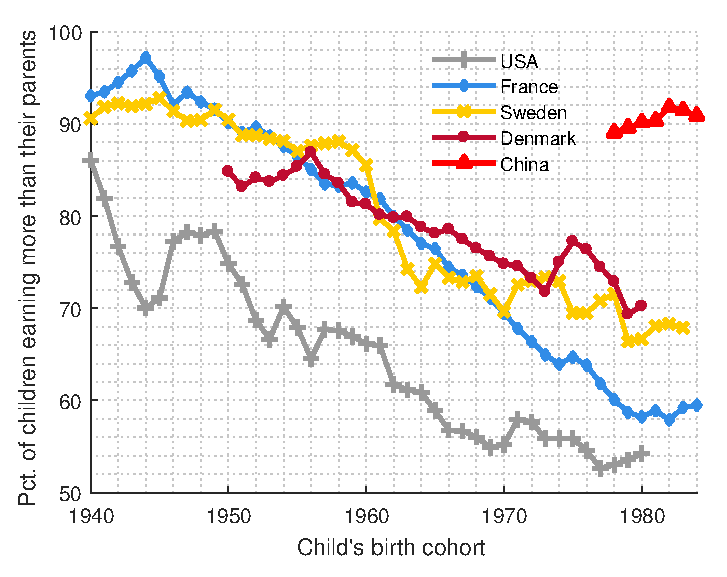
\includegraphics[width=1.0\textwidth] {./figs/countries2.eps}
\caption{Estimated rate of absolute mobility in the United States, France, Sweden, Denmark and China assuming the bivariate log-normal model and assuming fixed RRS of $0.3$~\citep{chetty2014land}, $0.42$~\citep{lefranc2005intergenerational}, $0.3$~\citep{bjorklund1997intergenerational}, $0.19$~\citep{landerso2016scandinavian} and $0.3$~\citep{fan2015great}, respectively.}
\flabel{countries}
\end{figure}

The results indicate that the decrease in absolute mobility rates found in the United States also occurred in France, Sweden and Denmark. However, in these countries, this decrease in mainly due to decreasing income growth rates rather than rising inequality. The results also partially echo stylized facts of relative mobility -- Denmark and Sweden are found as the most mobile of the countries analyzed apart from China, and the United States as the least.

The case of China is unique in comparison to the other countries analyzed. The estimated high absolute mobility likely reflects the high growth rates of the Chinese economy. The absolute mobility remains at such levels despite high income inequality rates~\citep{piketty2017capital} and is reinforced by the low relative intergenerational mobility~\citep{corak2013income,fan2015great} (see~\sref{theory}). \AAA{This sounds like speculation or one of many possible narratives.}

\subsection{Absolute and relative intergenerational mobility}
\label{sec:theory}

\AAA{I think this section would work better immediately after the results, i.e. as 3.1.}

Having established the model's empirical soundness, we can use its properties to further study the measures of mobility -- $A$, $R_1$ and $R_2$. Eqs.~(\ref{eq:abs2}--\ref{eq:abs3}) demonstrate that the rate of absolute mobility can be explicitly described as a function of the relative mobility measures $R_1$ and $R_2$.~\fref{relat} shows $A$ as a function of $R_1$ and $R_2$ for different birth cohorts in the United States. It shows that the bivariate normal model -- with positive income growth and inequality changes consistent with data, but absent other effects -- predicts an \textit{inverse} relationship between absolute and relative mobility.

\begin{figure}[!htb]
\centering
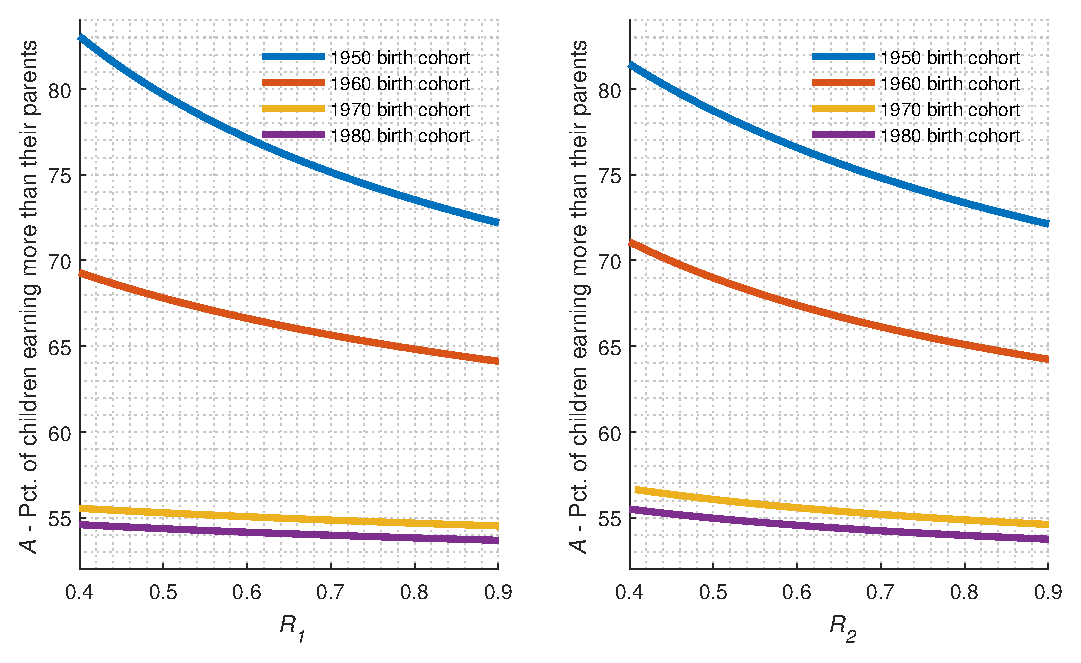
\includegraphics[width=1.0\textwidth] {./figs/R1_R2.eps}
\caption{The theoretical relationship between the rate of absolute mobility, $R_1$ (left) and $R_2$ (right), assuming the bivariate normal log-incomes model for different birth cohorts in the United States. This demonstrates the inverse relationship between absolute and relative mobility measures. \AAA{We don't need the verbal vertical axis titles.}}
\flabel{relat}
\end{figure}

\Pref{prop2} illustrates that the rate of absolute mobility increases with increasing income growth and decreases with increasing income inequality, as described by~\citet{chetty2017fading}. However, it also demonstrates that an additional mechanism can be at play, since the rate of absolute mobility decreases with increasing relative mobility. \AAA{Maybe a table of directional dependencies of $A$ on other quantities would be a useful addition, e.g. $\beta\uparrow$, $A\downarrow$, etc.} The direct implication is that if the relative mobility in the United States had been decreasing during the past few decades, as some argue~\citep{aaronson2008intergenerational,putnam2012growing}, the decrease in absolute mobility is less significant than reported by~\citet{chetty2017fading}. \AAA{I don't understand this sentence. If relative mobility has decreased, then absolute mobility should have increased ceteris paribus, with the implication that ceteris non paribus! Let's go through this on Skype. This is likely an important paragraph in the paper.}

\Fref{relat} seemingly stands in contrast to the findings about absolute intergenerational mobility in the United States, France, Sweden and Denmark (see~\fref{countries}), since the absolute and relative mobility in those countries were found to be ordered similarly. However, in practice, had the relative mobility in the United States been higher, the difference in absolute mobility rates with respect to the other countries would have become even larger.

The low relative intergenerational mobility in China contributes to its high levels of absolute intergenerational mobility. Had it been perfectly mobile in relative terms (\ie RRS of $0$), the estimated average absolute intergenerational mobility would have decreased by $4$ percentage points.

\section{Discussion}

The seemingly counterintuitive inverse theoretical relationship found between absolute and relative mobility stems from a fundamental conceptual difference between the two categories of mobility. It exposes the problems that can arise if both are treated as measuring similarly the same phenomenon. In particular, absolute mobility is very sensitive to across-the-board economic growth. For example, during the Middle Ages -- when relative mobility rates were low because social class and profession were predominantly inherited~\citep{goldthorpe1982social,clark2014also} -- even the slightest positive or negative income growth would result in very high or low absolute mobility. A misleading picture of intergenerational mobility may arise if the basic properties of these measures are overlooked. Therefore, empirically addressing this measure of intergenerational mobility requires careful delineation of the phenomena of interest and the manner in which quoted measures reflect them. In this study we exposed this particular property of the absolute mobility measure. \AAA{What property?}

From an empirical perspective, our findings imply that a model as simple as a bivariate log-normal distribution is satisfactory for describing the dynamics of absolute mobility. Thus, using available data on the marginal income distributions and on relative intergenerational mobility, one can produce estimates of absolute intergenerational mobility without the need for high-quality panel data sets, which remain unavailable in most countries.

\clearpage

\doublespacing
\bibliography{mobmob}

\clearpage

%\doublespacing

\appendix

\section{Proofs}
\label{app:appA}

\subsection{Proof of \preflong{prop1}}

First, by definition, the correlation $\rho$, between $X_p$ and $X_c$ equals to their covariance, divided by $\sigma_p\sigma_c$

\be
\rho = \frac{\text{Cov}\left[X_p,X_c\right]}{\sigma_p\sigma_c}\,.
\ee

$\beta$ can be directly calculated as follows, by the linear regression slope definition:

\be
\beta = \frac{\sum_{i=1}^{N} {\left(X_p^i - \bar{X}_p\right)\left(X_c^i - \bar{X}_c\right)}}{\sum_{i=1}^{N} {\left(X_p^i - \bar{X}_p\right)}}\,,
\ee
where $\bar{X}_p$ and $\bar{X}_c$ are the average parents and children log-incomes, respectively.

It follows that 
\be
\beta = \frac{\text{Cov}\left[X_p,X_c\right]}{\sigma_p^2}\,.
\ee

We immediately obtain

\be
\beta = \frac{\sigma_c}{\sigma_p}\rho
\ee

and therefore

\be
1-\beta = R_1 = 1-\frac{\sigma_c}{\sigma_p}\rho
\ee

\qed

\subsection{Proof of \preflong{prop2}}

We start by defining a new random variable $Z = X_c-X_p$. It follows that calculating $A$ is equivalent to calculating the probability $P\left(Z>0\right)$.

Subtracting two dependent normal distributions yields that

\be
Z \sim \mathcal{N}\left(\mu_c - \mu_p,\sigma_p^2 + \sigma_c^2 - 2\text{Cov}\left[X_p,X_c\right]\right)\,,
\ee

so according to \pref{prop1}

\be
Z \sim \mathcal{N}\left(\mu_c - \mu_p,\sigma_p^2\left(1-2\beta\right) + \sigma_c^2\right)\,.
\ee

If follows that

\be
\frac{Z - \left(\mu_c - \mu_p\right)}{\sqrt{\sigma_p^2\left(1-2\beta\right) + \sigma_c^2}} \sim \mathcal{N}\left(0,1\right)\,,
\ee

so we can now write

\be
\begin{split}
&P\left(Z>0\right) = \\ & P\left(\frac{Z - (\mu_c - \mu_p)}{\sqrt{\sigma_p^2\left(1-2\beta\right) + \sigma_c^2}} > -\frac{\mu_c - \mu_p}{\sqrt{\sigma_p^2\left(1-2\beta\right) + \sigma_c^2}} \right) = \\ &\Phi\left(\frac{\mu_c - \mu_p}{\sqrt{\sigma_p^2\left(1 - 2\beta\right) + \sigma_c^2}}\right) \,,
\end{split}
\ee
where $\Phi$ is the cumulative distribution function of the standard normal distribution.

\qed

\subsection{Proof of \creflong{coro1}}

For the bivariate log-normal model it is known that~\citep{trivedi2007copula}

\be
1-R_2 = \frac{6\arcsin{\frac{\rho}{2}}}{\pi}\,.
\ee

hence, using~\eref{beta_rho}

\be
R_2 = 1- \frac{6\arcsin{\frac{\sigma_p\beta}{2\sigma_c}}}{\pi}\,.
\ee

Substituting into~\eref{abs2} we obtain

\be
A = \Phi\left(\frac{\mu_c - \mu_p}{\sqrt{\sigma_p^2\left(1 - \frac{4\sigma_c}{\sigma_p}\sin{\left(\frac{\pi\left(1-R_2\right)}{6}\right)}\right) + \sigma_c^2}}\right) \,.
\ee

\qed

\subsection{Proof of \preflong{prop3}}

Following~\eref{abs2}

\be
A = \Phi\left(\frac{\mu_c - \mu_p}{\sqrt{\sigma_p^2\left(1 - 2\beta\right) + \sigma_c^2}}\right) \,.
\ee

Following~\eref{tildeA}

\be
\tilde{A} = \Phi\left(\frac{\mu_c-\mu_p}{\sigma_c} \right)
\ee

Therefore

\be
\tilde{A}=A \iff \frac{\mu_c - \mu_p}{\sqrt{\sigma_p^2\left(1 - 2\beta\right) + \sigma_c^2}} = \pm\frac{\mu_c-\mu_p}{\sigma_c}\,.
\ee

We then obtain

\be
\frac{\mu_c - \mu_p}{\sqrt{\sigma_p^2\left(1 - 2\beta\right) + \sigma_c^2}} = \pm\frac{\mu_c-\mu_p}{\sigma_c} \iff \sigma_c = \pm\sqrt{\sigma_p^2\left(1 - 2\beta\right) + \sigma_c^2} \iff \beta = \frac{1}{2}\,.
\ee

\qed

\section{Model robustness check}
\label{app:appB}

Our analysis was done for a bivariate log-normal model, assuming the marginal log-income distributions are normal and that their copula is Gaussian. This enables the derivation of \eref{abs2}, useful for investigating the relationship between absolute and relative mobility. This model for the joint income distributions of parents and children was found as unsatisfactory for some applications~\citep{bonhomme2009assessing}. Therefore, we wish to check how robust is this model when compared to other possible models, specifically applying it for calculating absolute mobility.

For that purpose we assume two possible shapes for the marginal income distributions -- log-normal and gamma, both used in numerous studies as approximations of empirical income distributions~\citep{salem1974convenient,pinkovskiy2009parametric}. The historical parameters for the marginal distributions were calculated using data for the pre-tax national income per adult in the United States and the income share data~\citep{WID2017}, as described in~\ref{sec:results}.

In addition, we assume four possible copula forms -- Gaussian, Clayton, Gumbel and Plackett. The reader is referred to~\citet{trivedi2007copula} and~\citet{bonhomme2009assessing} for a discussion in different uses of the different copula forms and their mathematical properties.

We test eight cases -- assuming each copula form and assuming log-normal and gamma marginal distributions. For each copula choice we also calculate the copula dependence parameter $\theta$~\citep{trivedi2007copula}, so it produces a rank-rank slope of $0.3$~\citep{chetty2014land}. For each case we calculate its root-mean-square deviation (RMSD) from the data and the relative absolute error (RAE).

The results of the robustness check are presented in~\tref{robust}. They show that using the log-normal marginal distributions yields consistently better results than when using gamma marginal distributions. In addition, the result were essentially independent of the copula form choice. None of the eight possible combinations of marginal distribution and copula stood out in comparison to the others.

\begin{table}[!htb]
\ra{1.1}
\centering
\captionof{table}{Model robustness check results}\tlabel{robust}
\begin{tabular}{@{}llcc@{}}\toprule[1.5pt]
Marginal distribution & Copula & RMSD & RAE\\
\midrule[1.5pt]
\multirow{ 4}{*}{Log-normal}
& Gaussian & 0.06 & 0.42\\
& Clayton & 0.06 & 0.43\\
& Gumbel &  0.06 & 0.39\\
& Plackett & 0.06 & 0.42\\
\midrule[1.5pt]
\multirow{ 4}{*}{Gamma}
& Gaussian  & 0.10 & 0.76\\
& Clayton  & 0.10 & 0.80\\
& Gumbel  & 0.09 & 0.67\\
& Plackett & 0.09 & 0.72\\
\bottomrule[1.5pt]
\end{tabular}
\end{table}

\Fref{copulas1} depicts the absolute intergenerational mobility resulting in each of the eight combinations in comparison to data. It illustrates the results presented in~\tref{robust} -- particularly that the difference between the various copula forms is very small and that the log-normal approximation provides a much better description of the absolute mobility dynamics than the gamma distribution approximation.

\begin{figure}[!htb]
\centering
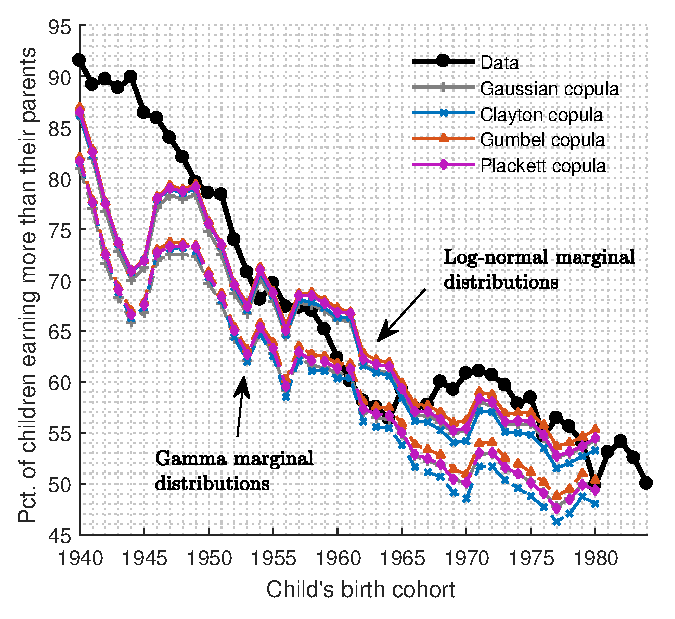
\includegraphics[width=1.0\textwidth]{./figs/copulas3.eps}
\caption{A comparison between the measured (black) and calculated absolute mobility for different copula forms using log-normal marginal distributions (solid lines) and using gamma marginal distributions (dashed lines).}
\flabel{copulas1}
\end{figure}

The robustness check shows that the Gaussian copula with log-normal marginal distributions, \ie the bivariate log-normal model, provides results which are no worse than any other combination. We therefore conclude that for the purpose of modeling the dynamics of absolute mobility, the bivariate log-normal model is indeed a good model.

\end{document}